\documentclass[../../main]{subfiles}

\begin{document}
\chapter{数ベクトル空間}
\label{chapter:numerical_vector_space}

\begin{lead}
  \cref{chapter:numerical_vector_space}では,数ベクトル空間における直交性と最良近似の関係を説明する.
\end{lead}

\section{直交射影}

本節では,あるベクトルを他のベクトルの線型結合で近似する手法を説明する.
特に断りのない限り,\cref{chapter:numerical_vector_space}において\(\numset{K}\)は\(\numset{R}\)か\(\numset{C}\)を意味し,
\(\innerp{\holder}{\holder}\)は\(\numset{K}^n\)の標準内積を意味する.また
\[
  \vnorm{\vect{x}} = \sqrt{\innerp{\vect{x}}{\vect{x}}}
  = \sqrt{\abs{x_1}^2+\dots+\abs{x_n}^2}
  \quad(\vect{x}=\trps{\matrice{x_1 & \cdots & x_n}}\in\numset{K}^n)
\]
とする\index{\(\vnorm{\holder}\)}.

\subsection{直交射影}

\(\numset{K}^n\)のベクトル\(\vect{x}\),部分空間\(V\)が与えられたとき,\(V\)の元で\(\vect{x}\)に最も近いベクトル,すなわち,距離\(\vnorm{\vect{x}-\vect{m}}\)を最小にする\(\vect{m}\in V\)について考えよう.

\begin{figure}[htbp]
  \centering
  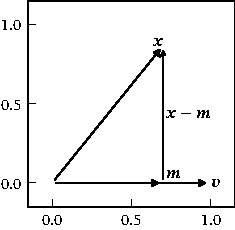
\includegraphics{proj2d.pdf}
  \caption{\(V=\spannedby\Set{\vect{v}}\)の元で\(\vect{x}\)に最も近いベクトル\(\vect{m}\)の様子.}
  \label{figure:proj2d}
\end{figure}

\(\numset{K}^n\)が平面\(\numset{R}^2\)で,\(V\)があるベクトル\(\vect{v}\neq\zvec\)により生成される直線\(\spannedby\Set{\vect{v}}\)の場合について,\(\vect{m}\)を図示したのが\cref{figure:proj2d}である.
\cref{figure:proj2d}を見ると,\(\vect{x}-\vect{m}\)は\(\vect{v}\)と直交しているのが分かる.

一般の部分空間\(V\subset\numset{K}^n\)についても,直交性は最良近似を特徴づける.証明へと入る前に,便利な記法を2つ定義しておく.

\begin{definition}{\(\argmin\),\(\argmax\)}{argmin_argmax}\index{あーぎゅみん@\(\argmin\)}\index{あーぎゅまっくす@\(\argmax\)}
  \(X\)を集合とする.集合\(S\subset X\)と関数\(f\colon X\to\numset{R}\)に対して,\(S\)の部分集合\(\argmin_{x\in S}f(x)\),\(\argmax_{x\in S}f(x)\)を以下の通り定義する.
  \begin{gather*}
    \argmin_{x\in S}f(x) = \Set{x\in S\given\text{任意の\(y\in S\)に対して\(f(y)\geq f(x)\)}}, \\
    \argmax_{x\in S}f(x) = \Set{x\in S\given\text{任意の\(y\in S\)に対して\(f(y)\leq f(x)\)}}
  \end{gather*}
\end{definition}

\cref{definition:argmin_argmax}からただちに,次のことが分かる.

\begin{proposition}{}{}
  \(S\)の元\(a\)に関する以下の条件は同値であり,同様のことが\(\argmax\)についても成り立つ.
  \begin{enumerate}
    \item \(a\in\argmin_{x\in S}f(x)\)である
    \item \(f(a)\)は集合\(\Set{f(x)\given x\in S}\)の下限であり,よって最小元でもある
  \end{enumerate}
\end{proposition}

\begin{example}
  \(\argmin_{x\in\coival{0}{\infty}}\exp(-x)=\argmax_{x\in\coival{0}{\infty}}\exp(x)=\emptyset\)である.
  また\(\argmin_{x\in\numset{R}}\abs{\sin(x)}=\Set{n\krez\given n\in\numset{Z}}\)である.
\end{example}

\begin{figure}[htbp]
  \centering
  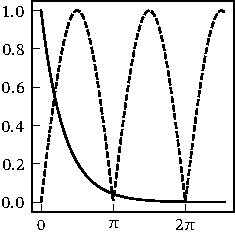
\includegraphics{argmin.pdf}
  \caption{\(\exp(-x)\)と\(\abs{\sin(x)}\)のグラフ.\(\exp(-x)\to 0\)(\(x\to\infty\))であるが,\(\exp(-x)=0\)となる実数\(x\)は存在しないことに注意.}
\end{figure}

\(\numset{K}=\numset{R}\)の場合も同様に証明できるので,\cref{proposition:finite_projection}まで証明では\(\numset{K}=\numset{C}\)を仮定する.また,部分空間が\(\Set{\zvec}\)でないことも仮定する.

\begin{proposition}{}{finite_convex_projection}
  \(\vect{x}\in\numset{K}^n\)かつ,\(V\)は\(\numset{K}^n\)の部分空間とする.
  このとき,\(\argmin_{\vect{y}\in V}\vnorm{\vect{x}-\vect{y}}\)はただ1つの元からなる集合である.
\end{proposition}

\begin{proof}
  \(\basis{B}=\Set{\vect{e}_1,\dots,\vect{e}_m}\)を\(V\)の正規直交基底とすると,
  \(V\)は\(\Set{z_1\vect{e}_1+\dots+z_m\vect{e}_m\given z_1,\dots,z_m\in\numset{C}}\)と書ける.
  したがって,\(f(z_1,\dots,z_m)=\vnorm{\vect{x}-(z_1\vect{e}_1+\dots+z_m\vect{e}_m)}\)(\(z_1,\dots,z_m\in\numset{C}\))とおくと
  \[
    \argmin_{\vect{y}\in V}\vnorm{\vect{x}-\vect{y}} = \Set*{z_1\vect{e}_1+\dots+z_m\vect{e}_m\given\trps{\matrice{z_1 & \cdots & z_m}}\in\argmin_{\vect{z}\in\numset{C}^m}f(\vect{z})}
  \]
  である.

  \(\argmin_{\vect{z}\in\numset{C}^m}f(\vect{z})\)を求める.\(\basis{B}\)は正規直交基底だから
  \[
    \vnorm*{\sum_{i=1}^mz_i\vect{e}_i}^2 = \innerp*{\sum_{i=1}^mz_i\vect{e}_i}{\sum_{j=1}^mz_j\vect{e}_j}
    = \sum_{i=1}^m\sum_{j=1}^mz_i\conj{z_j}\innerp{\vect{e}_i}{\vect{e}_j}
    = \sum_{i=1}^m\sum_{j=1}^mz_i\conj{z_j}\kdelta{i}{j}
    = \sum_{i=1}^m\abs{z_i}^2
  \]
  となる.したがって(\(\sum_{k=1}^m\)を\(\sum\)と略記すると)
  \begin{align*}
    f(\vect{z})^2 &= \vnorm*{\vect{x}-\sum z_k\vect{e}_k}^2 = \vnorm{\vect{x}}^2-2\rpart\innerp*{\vect{x}}{\sum z_k\vect{e}_k}+\vnorm*{\sum z_k\vect{e}_k}^2 \\
    &= \vnorm{\vect{x}}^2-2\sum\rpart[\conj{z_k}\innerp{\vect{x}}{\vect{e}_k}]+\sum\abs{z_k}^2
  \end{align*}
  である.よって,\(f(\vect{z})^2\)は\(s_k=\rpart z_k\)と\(t_k=\ipart z_k\)の式で
  \begin{align*}
    f(\vect{z})^2 &= \vnorm{\vect{x}}^2+\sum(-2\rpart[(s_k-\iuni t_k)\innerp{\vect{x}}{\vect{e}_k}]+s_k^2+t_k^2) \\
    &= \vnorm{\vect{x}}^2+\sum(-2(s_k\rpart\innerp{\vect{x}}{\vect{e}_k}+t_k\ipart\innerp{\vect{x}}{\vect{e}_k})+s_k^2+t_k^2) \\
    &= \vnorm{\vect{x}}^2+\sum((s_k-\rpart\innerp{\vect{x}}{\vect{e}_k})^2+(t_k-\ipart\innerp{\vect{x}}{\vect{e}_k})^2-\abs{\innerp{\vect{x}}{\vect{e}_k}}^2)
  \end{align*}
  と書けるので,次式が成立する.
  \begin{equation}
    \label{equation:pre_bessels_inequality}
    f(\vect{z})^2 = \vnorm{\vect{x}}^2+\sum_{k=1}^m\abs{z_k-\innerp{\vect{x}}{\vect{e}_k}}^2-\sum_{k=1}^m\abs{\innerp{\vect{x}}{\vect{e}_k}}^2
  \end{equation}

  \cref{equation:pre_bessels_inequality}より\(\argmin_{\vect{z}\in\numset{C}^m}f(\vect{z})=\Set{\trps{\rowvect{\innerp{\vect{x}}{\vect{e}_1} & \cdots & \innerp{\vect{x}}{\vect{e}_m}}}}\)であるから,
  \(\argmin_{\vect{y}\in V}\vnorm{\vect{x}-\vect{y}}=\Set{\innerp{\vect{x}}{\vect{e}_1}\vect{e}_1+\dots+\innerp{\vect{x}}{\vect{e}_m}\vect{e}_m}\)である.
\end{proof}

なお,\cref{proposition:finite_convex_projection}は部分空間よりも少し広い対象(閉凸集合)へと一般化できるのだが,そのことは\cref{xr-chapter:hilbert_space}であらためて扱う.

\begin{proposition}{}{weak_finite_projection}
  \(\vect{x}\in\numset{K}^n\)かつ,\(V\)は\(\numset{K}^n\)の部分空間とする.
  \(V\)のある元\(\vect{m}\)が任意の\(\vect{y}\in V\)に対して\(\innerp{\vect{x}-\vect{m}}{\vect{y}}=0\)を満たすとき,
  \(\vect{m}\in\argmin_{\vect{y}\in V}\vnorm{\vect{x}-\vect{y}}\)である.
\end{proposition}

\begin{proof}
  任意に\(\vect{y}\in V\)をとり,\(\vect{e}=\vect{y}-\vect{m}\)とおく.すると,\(\innerp{\vect{x}-\vect{m}}{\vect{e}}=0\)より
  \(\vnorm{\vect{x}-\vect{y}}^2=\vnorm{\vect{x}-\vect{m}-\vect{e}}^2=\vnorm{\vect{x}-\vect{m}}^2-2\rpart\innerp{\vect{x}-\vect{m}}{\vect{e}}+\vnorm{\vect{e}}^2=\vnorm{\vect{x}-\vect{m}}^2+\vnorm{\vect{e}}^2\)
  が成立する.よって\(\vnorm{\vect{x}-\vect{y}}^2\geq\vnorm{\vect{x}-\vect{m}}^2\)だから,\(\vect{m}\in\argmin_{\vect{y}\in V}\vnorm{\vect{x}-\vect{y}}\)である.
\end{proof}

\cref{proposition:weak_finite_projection}からは,仮定「任意の\(\vect{y}\in V\)に対して\(\innerp{\vect{x}-\vect{m}}{\vect{y}}=0\)」を満たす\(\vect{m}\in V\)が存在するかどうかは分からない.
しかし実は,仮定を満たす\(\vect{m}\)は一意に存在し,それは\(\argmin_{\vect{y}\in V}\vnorm{\vect{x}-\vect{y}}\)のただ1つの元である.

\begin{proposition}{}{finite_projection}
  \(\vect{x}\in\numset{K}^n\)かつ,\(V\)は\(\numset{K}^n\)の部分空間とする.
  このとき,\(V\)の元\(\vect{m}\)に関する以下の条件は同値であり,条件を満たす\(\vect{m}\)はただ1つ存在する.
  \begin{enumerate}
    \item \(\vect{m}\in\argmin_{\vect{y}\in V}\vnorm{\vect{x}-\vect{y}}\)である
    \item 任意の\(\vect{y}\in V\)に対して\(\innerp{\vect{x}-\vect{m}}{\vect{y}}=0\)である
  \end{enumerate}
\end{proposition}

\begin{proof}
  \cref{proposition:finite_convex_projection}より,\(\vect{n}\in\argmin_{\vect{y}\in V}\vnorm{\vect{x}-\vect{y}}\)を満たす\(\vect{n}\)がただ1つ存在する.
  そして\cref{proposition:weak_finite_projection}より,\(\vect{m}\in V\)が任意の\(\vect{y}\in V\)に対して\(\innerp{\vect{x}-\vect{m}}{\vect{y}}=0\)を満たすなら\(\vect{m}=\vect{n}\)である.

  したがって,\(\vect{n}\)がすべての\(\vect{v}\in V\)に対して\(\innerp{\vect{x}-\vect{n}}{\vect{v}}=0\)を満たすことを示せばよい.それには\(\vnorm{\vect{v}}=1\)のときについて示せば十分である.
  \(\vect{n}\)の定義から,関数\(e(z)=\vnorm{\vect{x}-(\vect{n}+z\vect{v})}^2-\vnorm{\vect{x}-\vect{n}}^2\)(\(z\in\numset{C}\))は負の値をとらない.一方,\(x=\rpart z\),\(y=\ipart z\)とおくと
  \begin{align*}
    e(z) &= \vnorm{\vect{x}-\vect{n}-z\vect{v}}^2-\vnorm{\vect{x}-\vect{n}}^2
    = -2\rpart[(x-\iuni y)\innerp{\vect{x}-\vect{n}}{\vect{v}}]+\abs{z}^2\vnorm{\vect{v}}^2 \\
    &= -2(x\rpart\innerp{\vect{x}-\vect{n}}{\vect{v}}+y\ipart\innerp{\vect{x}-\vect{n}}{\vect{v}})+x^2+y^2 \\
    &= (x-\rpart\innerp{\vect{x}-\vect{n}}{\vect{v}})^2+(y-\ipart\innerp{\vect{x}-\vect{n}}{\vect{v}})^2-\abs{\innerp{\vect{x}-\vect{n}}{\vect{v}}}^2 \\
    &= \abs{z-\innerp{\vect{x}-\vect{n}}{\vect{v}}}^2-\abs{\innerp{\vect{x}-\vect{n}}{\vect{v}}}^2
  \end{align*}
  なので\(\abs{\innerp{\vect{x}-\vect{n}}{\vect{v}}}^2=-e(\innerp{\vect{x}-\vect{n}}{\vect{v}})\leq 0\),よって\(\innerp{\vect{x}-\vect{n}}{\vect{v}}=0\)である.
\end{proof}

\begin{definition}{直交射影}{finite_projection}\index{ちょっこうしゃえい@直交射影!かずべくとるくうかんじょうの@数ベクトル空間}\index{ぷろじぇくしょん@\(\proj_V(\vect{x})\)}
  \cref{proposition:finite_projection}の\(\vect{m}\)を\(\vect{x}\)の\(V\)への\termdef{直交射影}(orthogonal projection)といい,\(\proj_V(\vect{x})\)と表す.
\end{definition}

\begin{figure}[htbp]
  \centering
  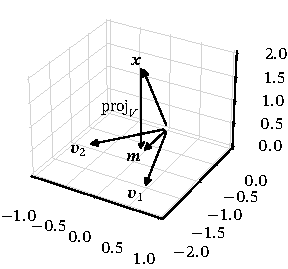
\includegraphics{proj3d.pdf}
  \caption{\(\vect{x}\)の\(V=\spannedby\Set{\vect{v}_1,\vect{v}_2}\)への直交射影\(\vect{m}=\proj_V(\vect{x})\)の模式図.}
\end{figure}

\begin{example}
  \(\vect{v}_1=\trps{\rowvect{1 & 1 & 1}}\),\(\vect{v}_2=\trps{\rowvect{2 & -1+\iuni\sqrt{3} & -1-\iuni\sqrt{3}}}\)とし,
  \(\numset{C}^3\)の部分空間\(V\)を\(V=\spannedby\Set{\vect{v}_1,\vect{v}_2}\)で定義する.
  このとき\(\innerp{\vect{v}_1}{\vect{v}_2}=0\),\(\vnorm{\vect{v}_1}=\sqrt{3}\),\(\vnorm{\vect{v}_2}=\sqrt{12}\)だから,
  集合\(\Set{\vect{v}_1/\sqrt{3},\vect{v}_2/\sqrt{12}}\)は\(V\)の正規直交基底である.よって
  \[
    \proj_V(\vect{x}) = \innerp*{\vect{x}}{\frac{\vect{v}_1}{\sqrt{3}}}\frac{\vect{v}_1}{\sqrt{3}}+\innerp*{\vect{x}}{\frac{\vect{v}_2}{\sqrt{12}}}\frac{\vect{v}_2}{\sqrt{12}}
    = \frac{\innerp{\vect{x}}{\vect{v}_1}}{3}\vect{v}_1+\frac{\innerp{\vect{x}}{\vect{v}_2}}{12}\vect{v}_2
  \]
  である.
\end{example}

\begin{proposition}{}{}
  \(\numset{K}^n\)の任意の部分空間\(V\)について,写像\(\proj_V\colon\numset{K}^n\to V\)は線型写像である.
\end{proposition}

\begin{proof}
  \(s,t\in\numset{K}\),\(\vect{x},\vect{y}\in\numset{K}^n\)を任意にとり,\(\vect{m}=s\proj_V(\vect{x})+t\proj_V(\vect{y})\)とおく.
  このとき,任意の\(\vect{v}\in V\)に対して\(\innerp{s\vect{x}+t\vect{y}-\vect{m}}{\vect{v}}=s\innerp{\vect{x}-\proj_V(\vect{x})}{\vect{v}}+t\innerp{\vect{y}-\proj_V(\vect{y})}{\vect{v}}=s0+t0=0\)となるので,
  \(\proj_V(s\vect{x}+t\vect{y})=\vect{m}\)である.よって,\(\proj_V\)は線型写像である.
\end{proof}

\subsection{直交補空間}

\begin{definition}{直交補空間}{numerical_perpendicular_complement}\index{ちょっこうほくうかん@直交補空間}\index{\(\pcomp{W}\)}\index{\(\pcomp[V]{W}\)}
  \(V\)は\(\numset{K}^n\)の部分空間とする.\(W\)が\(V\)の部分空間なら,集合
  \[
    X = \Set{\vect{v}\in V\given\text{任意の\(\vect{w}\in W\)に対して\(\innerp{\vect{v}}{\vect{w}}=0\)}}
  \]
  も\(V\)の部分空間になる.\(X\)を(\(V\)における)\(W\)の\termdef{直交補空間}(orthogonal complement)といい,\(\pcomp[V]{W}\)と表記する.誤解のおそれがなければ,\(\pcomp[V]{W}\)を\(\pcomp{W}\)とも書く.
\end{definition}

\begin{example}
  \(W=\spannedby\Set{\vect{e}_1,\vect{e}_2}\)を\(\numset{R}^3\)の2次元部分空間とする.
  このとき,\(\numset{R}^3\)における\(W\)の直交補空間は\(\vect{e}_1\)と\(\vect{e}_2\)に直交する\(\zvec\)でないベクトル\(\vect{e}_3\)で生成される直線\(\spannedby\Set{\vect{e}_3}\)である.
  特に\(\vect{e}_1\)と\(\vect{e}_2\)が直交するとき,集合\(\Set{\vect{e}_1,\vect{e}_2,\vect{e}_3}\)は\(\numset{R}^3\)の正規直交基底である.
\end{example}

\begin{figure}[htbp]
  \centering
  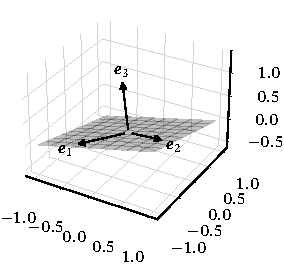
\includegraphics{orthogonal_complement.pdf}
  \caption{\(W\)と\(\vect{e}_1\),\(\vect{e}_2\),\(\vect{e}_3\)の様子.}
\end{figure}

\begin{proposition}{}{}
  \(V\)は\(\numset{K}^n\)の部分空間で,\(W\)は\(V\)の部分空間とする.このとき\(V=W\oplus\pcomp[V]{W}\)である.
\end{proposition}

\begin{proof}
  \(\vect{x}\in W\cap\pcomp{W}\)なら\(\innerp{\vect{x}}{\vect{x}}=0\)なので\(\vect{x}=\zvec\),よって\(W\cap\pcomp{W}=\Set{\zvec}\)である.
  また\cref{proposition:finite_projection}より,任意の\(\vect{x}\in V\)に対して\(\vect{x}-\proj_W(\vect{x})\in\pcomp{W}\),\(\vect{x}=\proj_W(\vect{x})+(\vect{x}-\proj_W(\vect{x}))\in W+\pcomp{W}\)である.
  したがって\(V=W\oplus\pcomp{W}\)である.
\end{proof}

\subsection{分析と合成}

\cref{proposition:finite_convex_projection}の証明では,\(\proj_V(\vect{x})\)の存在を示すために\(V\)の正規直交基底\(\basis{B}=\Set{\vect{e}_1,\dots,\vect{e}_m}\)を1つ選び,\(\proj_V(\vect{x})\)を\(\sum_{i=1}^m\innerp{\vect{x}}{\vect{e}_i}\vect{e}_i\)と表した.
一方で(特に信号解析では),\(\vect{x}\)の性質を調べるのに利用したい\(\numset{C}^n\)の正規直交基底\(\basis{B}=\Set{\vect{e}_1,\dots,\vect{e}_n}\)があって,
そこから部分空間\(V_m=\spannedby\Set{\vect{e}_1,\dots,\vect{e}_m}\)(\(m=1,\dots,n\))への直交射影\(\proj_{V_m}(\vect{x})\)を作ることも多い.そのような場合,直交射影は3つの操作に分解できる.

\begin{definition}{エルミート転置}{hermitian_transpose}\index{えるみーとてんち@エルミート転置}\index{ずいはんぎょうれつ@随伴行列|see{エルミート転置}}\index{えいち@\(\htrps{\mat{A}}\)}
  \(\mat{A}\)を\(m\times n\)複素行列とする.\(n\times m\)行列\(\conj{\trps{\mat{A}}}\)を\(\mat{A}\)の\termdef{エルミート転置}(Hermitian transpose)といい,\(\htrps{\mat{A}}\)と表す\footnotemark .
\end{definition}

\footnotetext{エルミート転置は\termdef{随伴行列}(adjoint matrix)と呼ばれることも多いが,別の行列を随伴行列と呼ぶ流儀もあり,まぎらわしい.そのため,本書ではエルミート転置で統一する.}

\(\mat{U}=\htrps{\rowvect{\vect{e}_1 & \cdots & \vect{e}_n}}\),\(\mat{\Lambda}=\begin{bsmallmatrix}\imat_m & \\ & \zmat_{n-m}\end{bsmallmatrix}=\diag(1,\dots,1,0,\dots,0)\)とおく.
このとき,任意の\(\vect{x}=\trps{\rowvect{x_1 & \cdots & x_n}}\in\numset{C}^n\)に対して
\[
  \mat{U}\vect{x} = \matrice*{\htrps{\vect{e}_1}\vect{x} \\ \vdots \\ \htrps{\vect{e}_n}\vect{x}}
  = \matrice*{\innerp{\vect{x}}{\vect{e}_1} \\ \vdots \\ \innerp{\vect{x}}{\vect{e}_n}},
  \quad\mat{\Lambda}\vect{x} = \matrice*{x_1 \\ \vdots \\ x_m \\ \zvec},
  \quad\htrps{\mat{U}}\vect{x} = \htrps{\mat{U}}\matrice*{x_1 \\ \vdots \\ x_n}
  = \sum_{i=1}^nx_i\vect{e}_i
\]
であるから
\[
  \htrps{\mat{U}}\mat{\Lambda}\mat{U}\vect{x} = \htrps{\mat{U}}\mat{\Lambda}\matrice*{\innerp{\vect{x}}{\vect{e}_1} \\ \vdots \\ \innerp{\vect{x}}{\vect{e}_n}}
  = \htrps{\mat{U}}\matrice*{\innerp{\vect{x}}{\vect{e}_1} \\ \vdots \\ \innerp{\vect{x}}{\vect{e}_m} \\ \zvec}
  = \sum_{i=1}^m\innerp{\vect{x}}{\vect{e}_i}\vect{e}_i
  = \proj_{V_m}(\vect{x})
\]
であり,\(\proj_{V_m}(\vect{x})=\htrps{\mat{U}}\mat{\Lambda}\mat{U}\vect{x}\)が成立する.言い換えれば,\(\proj_{V_m}\)は\(\numset{C}^n\)から\(\numset{C}^n\)への3つの写像
\(T(\vect{x})=\mat{U}\vect{x}\),\(L(\vect{x})=\mat{\Lambda}\vect{x}\),\(\synth{T}(\vect{x})=\htrps{\mat{U}}\vect{x}\)を用いて,\(\proj_{V_m}=\synth{T}LT\)と表せる.

\begin{definition}{正規行列,ユニタリ行列}{regular_and_unitary_matrix}\index{せいきぎょうれつ@正規行列}\index{ゆにたりぎょうれつ@ユニタリ行列}
  \(\mat{A}\)を\(n\)次複素正方行列とする.
  \begin{enumerate}
    \item \(\htrps{\mat{A}}\mat{A}=\mat{A}\htrps{\mat{A}}\)であるとき,\(\mat{A}\)を\termdef{正規行列}(normal matrix)という
    \item \(\htrps{\mat{A}}\mat{A}=\mat{A}\htrps{\mat{A}}=\imat\)であるとき(つまり\(\htrps{\mat{A}}=\mat{A}^{-1}\)であるとき),\(\mat{A}\)を\termdef{ユニタリ行列}(unitary matrix)という
  \end{enumerate}
\end{definition}

\cref{definition:regular_and_unitary_matrix}から,ユニタリ行列は正規行列である.また,次の命題が成立する.

\begin{proposition}{ユニタリ行列の性質}{}
  \(\mat{U}=\rowvect{\vect{u}_1 & \cdots & \vect{u}_n}\)を\(n\)次複素正方行列とする.このとき,以下の命題は同値である.
  \begin{enumerate}
    \item \(\mat{U}\)はユニタリ行列である
    \item 集合\(\Set{\vect{u}_1,\dots,\vect{u}_n}\)は\(\numset{C}^n\)の正規直交基底である
  \end{enumerate}
\end{proposition}

\begin{proof}
  \(\htrps{\mat{U}}\mat{U}=[\midx{a}{i}{j}]\)とおくと
  \[
    \htrps{\mat{U}}\mat{U} = \matrice*{\htrps{\vect{u}_1} \\ \vdots \\ \htrps{\vect{u}_n}}\matrice{\vect{u}_1 & \cdots & \vect{u}_n}
    = \matrice*{\htrps{\vect{u}_1}\vect{u}_1 & \cdots & \htrps{\vect{u}_1}\vect{u}_n \\ \vdots & \ddots & \vdots \\ \htrps{\vect{u}_n}\vect{u}_1 & \cdots & \htrps{\vect{u}_n}\vect{u}_n}
  \]
  なので\(\midx{a}{i}{j}=\htrps{\vect{u}_i}\vect{u}_j=\innerp{\vect{u}_j}{\vect{u}_i}\)である.よって,\(\mat{U}^{-1}=\htrps{\mat{U}}\)であることと,各\(i,j\in\Set{1,\dots,n}\)に対して\(\innerp{\vect{u}_i}{\vect{u}_j}=\kdelta{i}{j}\)であることは同値である.
\end{proof}

\subsection{スペクトル定理}

\section{最小2乗問題}

\subsection{最小2乗問題}

\subsection{特異値分解}

\subsection{擬似逆行列}

\section{離散フーリエ変換}

\section{多重解像度解析}

\section{主成分分析}
\begin{figure}[htbp]
  \begin{minipage}{\linewidth/2}
    \centering
    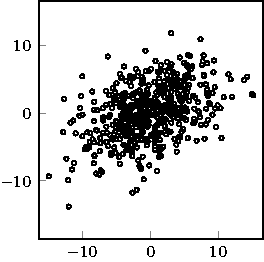
\includegraphics{scatter.pdf}
  \end{minipage}%
  \begin{minipage}{\linewidth/2}
    \centering
    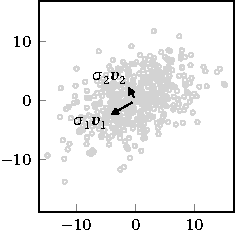
\includegraphics{pca.pdf}
  \end{minipage}
\end{figure}

\begin{subappendices}
\section{低ランク近似}
\end{subappendices}

\section*{演習問題}
\addcontentsline{toc}{section}{演習問題}

\end{document}
